\section{Experiments and Discussions}
\label{sec:results}
\subsection{SVR Based Occupancy Detection}
In this section, we illustrate how we measure error variation for
the proposed SVR model and discuss the effectiveness of applying
different number of features in this model.

\subsubsection{Experiments}
\begin{table}[!h]
\centering
    \begin{tabular}{lrrcrrcrr}
        \toprule
            & \multicolumn{2}{c}{$C=100$} && \multicolumn{2}{c}{$C=500$} && \multicolumn{2}{c}{$C=1000$} \\
        \cmidrule{2-3} \cmidrule{5-6} \cmidrule{8-9}
        \#Features &   \multicolumn{1}{c}{4} & \multicolumn{1}{c}{5} && \multicolumn{1}{c}{4} & \multicolumn{1}{c}{5} && \multicolumn{1}{c}{4} & \multicolumn{1}{c}{5}  \\
        \midrule
        Avg. error&0.721& 0.310   && 0.576 &  0.326   &&  0.550  &  0.348        \\
        Error~rate&31.1\%& 8.56\%  && 18.8\% &  8.89\%  &&  18.1\%  &  12.4\%        \\
        \bottomrule
    \end{tabular}
\caption{Training errors of SVR model using different numbers of features.}
\label{table:training}
\end{table}
\begin{table}[!h]
    \centering
    \begin{tabular}{lrrcrrcrr}
        \toprule
            & \multicolumn{2}{c}{$C=100$} && \multicolumn{2}{c}{$C=500$} && \multicolumn{2}{c}{$C=1000$} \\
        \cmidrule{2-3} \cmidrule{5-6} \cmidrule{8-9}
        \#Features &   \multicolumn{1}{c}{4} & \multicolumn{1}{c}{5} && \multicolumn{1}{c}{4} & \multicolumn{1}{c}{5} && \multicolumn{1}{c}{4} & \multicolumn{1}{c}{5}  \\
        \midrule
        Avg.~error&0.819& 0.317   && 0.694  &  0.330   &&  0.638  &  0.390        \\
        Error~rate&6.80\%& 2.64\%  && 5.78\% &  2.74\%  &&  5.32\%  &  3.25\%        \\
        \bottomrule
    \end{tabular}
    \caption{Validation errors of SVR model using different numbers
    of features.}
    \label{table:testing}
\end{table}

We evaluate the SVR detection model using
testing data set. Through a wide range of experiments, we learn radial
basis function kernel also known as Gaussian kernel works best in this
model. The two most important parameters in SVR model
are the penalty $C$ and the radius $\varepsilon$. For the confidence penalty,
the grid search algorithm \cite{Hsu2003} is performed for finding a confidence
penalty weight to work best.
It is widely known that to get an accurate performance in SVR model or any other machine
learning methods, the best approach is to enumerate a quantity of
combinations of parameters, and conduct experiments to drive the
result toward a better trend. During the process of seeking out the
best result for the model, the set of parameters is adjusted step by
step to obtain a model which has a better accuracy than the previous
one. After a batch of experiments for the model are conducted, we pick
out the parameters in the model that brings about the best
performance. Here we also want to highlight, that most of the time,
the parameters working best for a model sometimes can not be proved
theoretically, therefore confirmed parameters often are determined by
a great number of trials and experiments.

Table \rom{1} shows the training error statistics of the proposed SVR
model used for occupancy detection. Some comparisons between two sets
of features are apparently displayed from the results shown in this
table. Numerical simulation shows that $\varepsilon$ being equivalent
to 0.01 is a reliable choice for this SVR-based occupancy model. At
each sample point, the estimation error ${e_i}$ is defined as
${e_i} = \left| {O_i^{\textrm{SVR}} - O_i^{\textrm{EP}}} \right|$ where $O_i^{\textrm{SVR}}$
denotes the occupancy value obtained by the proposed SVR model and
$O_i^{\textrm{EP}}$ denotes the real value of occupancy generated from EnergyPlus. We calculate the average error and the error rate by
$\frac{1}{n}\sum\nolimits_n {{e_i}}$ and
$\frac{\text{average error}}{\text{full occupancy}}$,
respectively. Also, in this table different values of $C$ are tested
to seek out an accurate model for occupancy detection.

Table \rom{2} shows the validation error statistics of the proposed SVR model.
The reason why the 5-feature model performs better than the 4-feature
model for occupancy detection is that the 4-feature model suffers slightly in
under-fitting issue which results in a high bias. It is important to determine
the parameters which can maintain a balance between under-fitting and
over-fitting.


\subsubsection{Analysis}
\begin{figure}[h]
\begin{minipage}{\textwidth}
\centering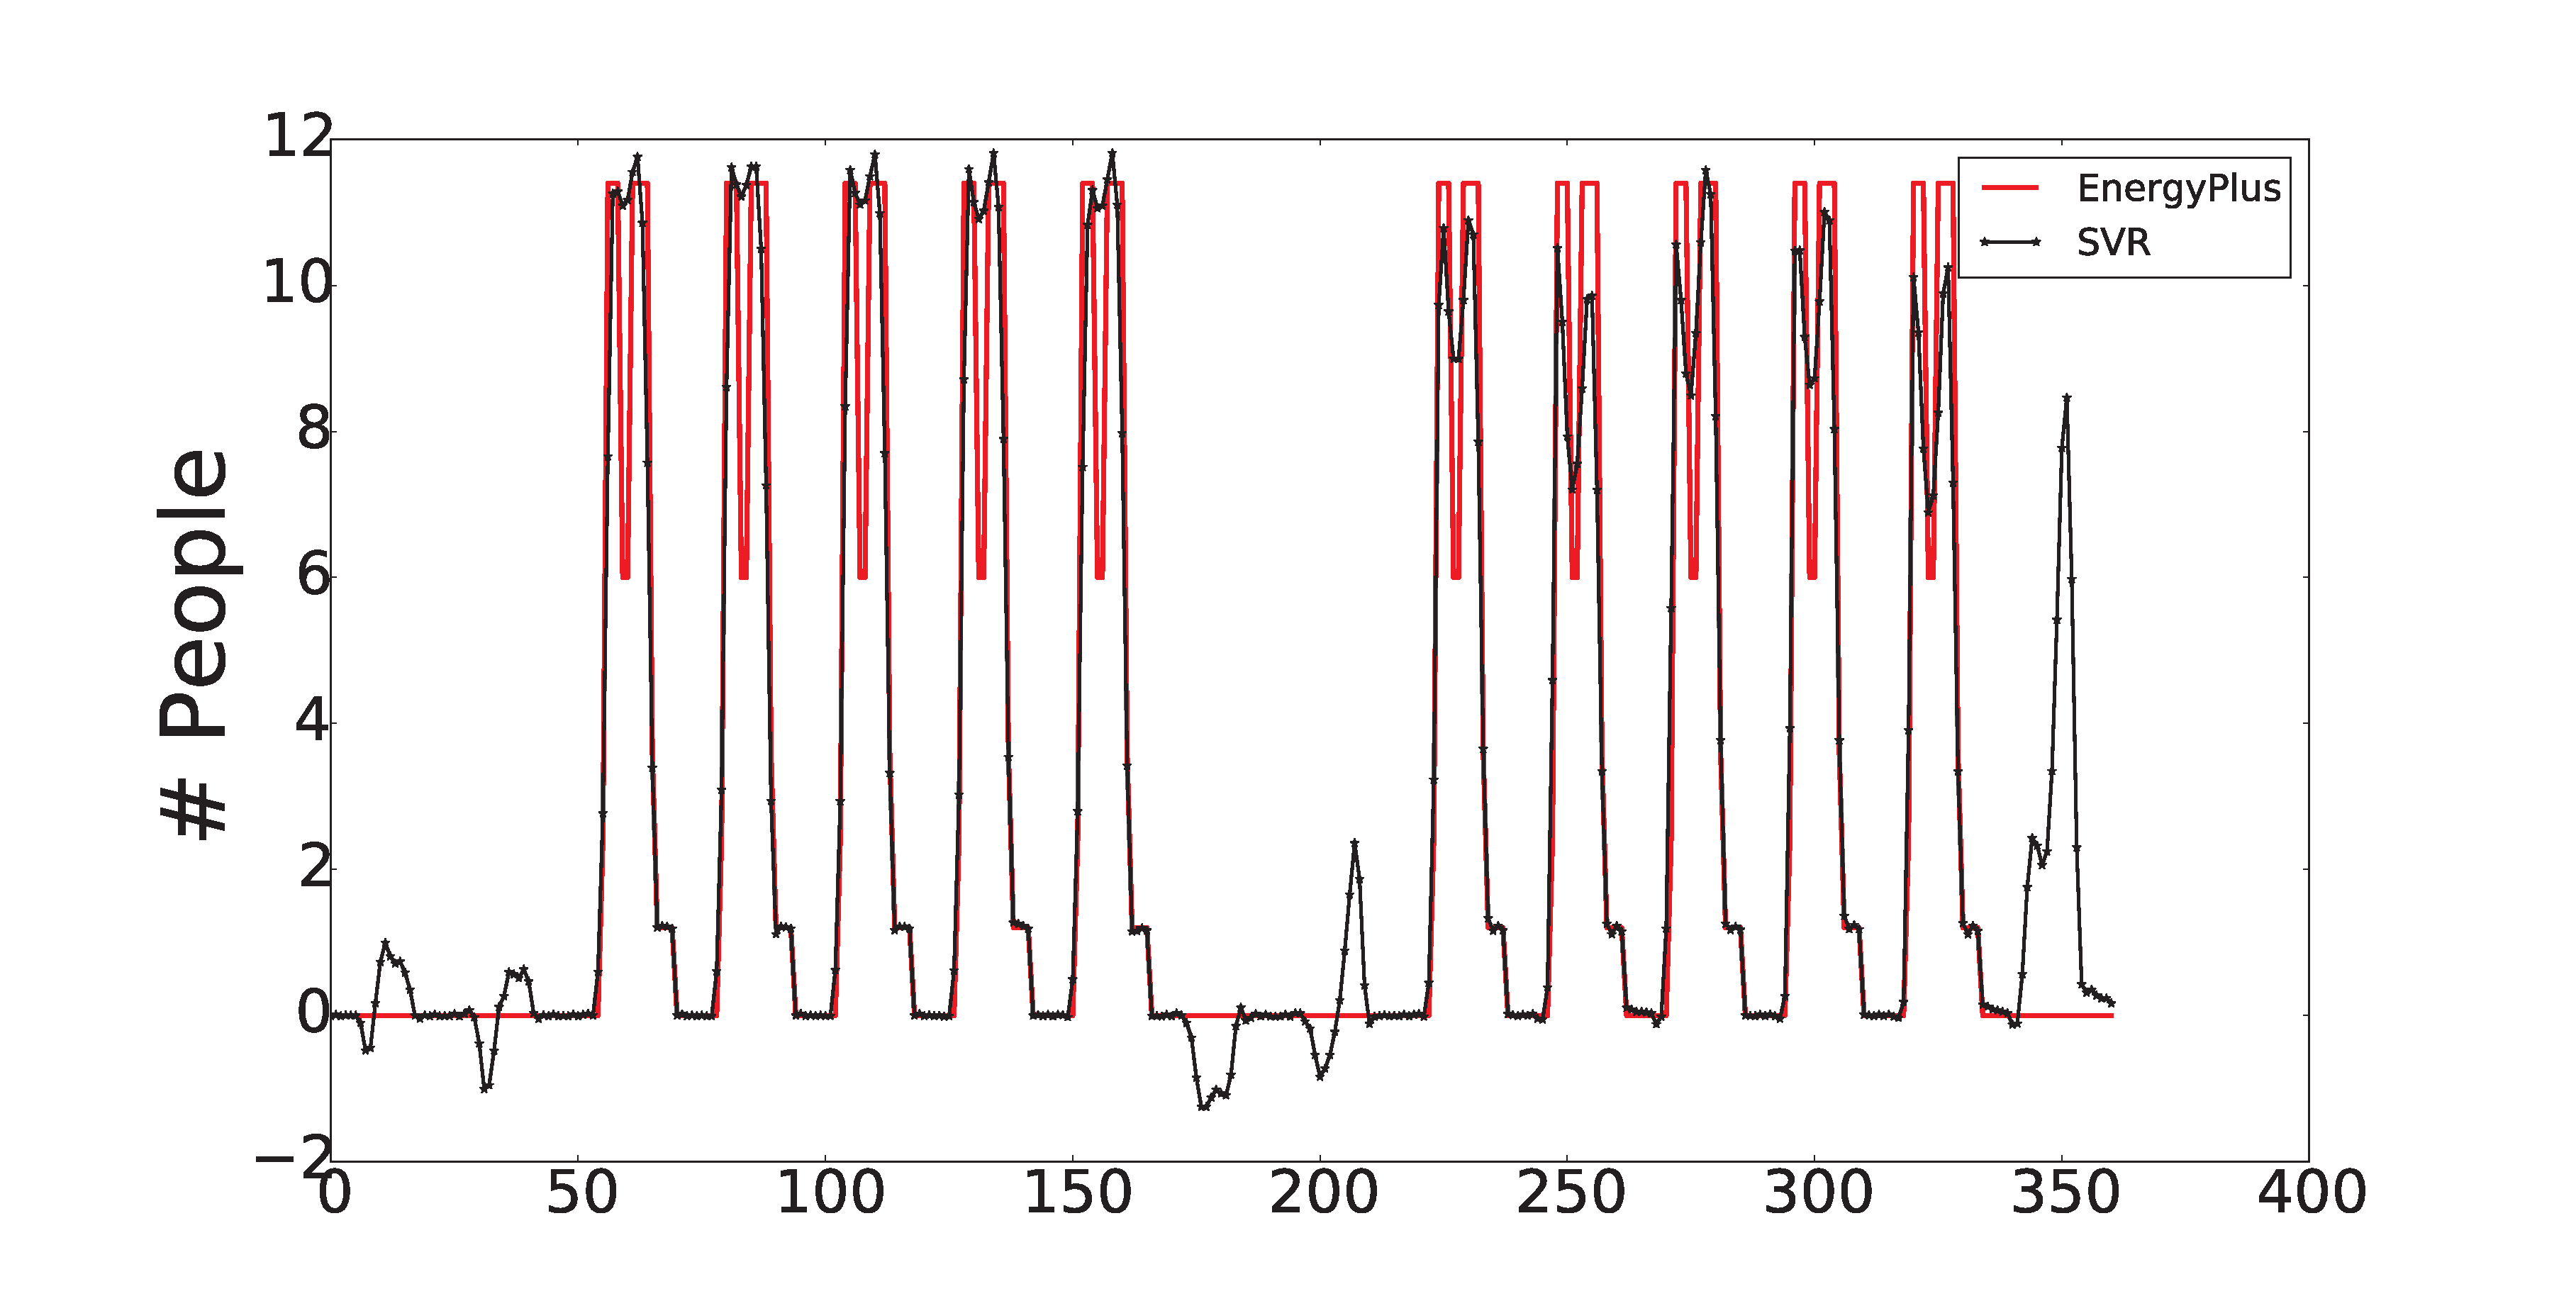
\includegraphics[width=5in]{./Pics/100C4Features.eps}
%\subcaption{}\label{fig:1a}
(a) 4 features.
\end{minipage}
\hfill

\vspace{3ex}

\noindent\begin{minipage}{\textwidth}
\centering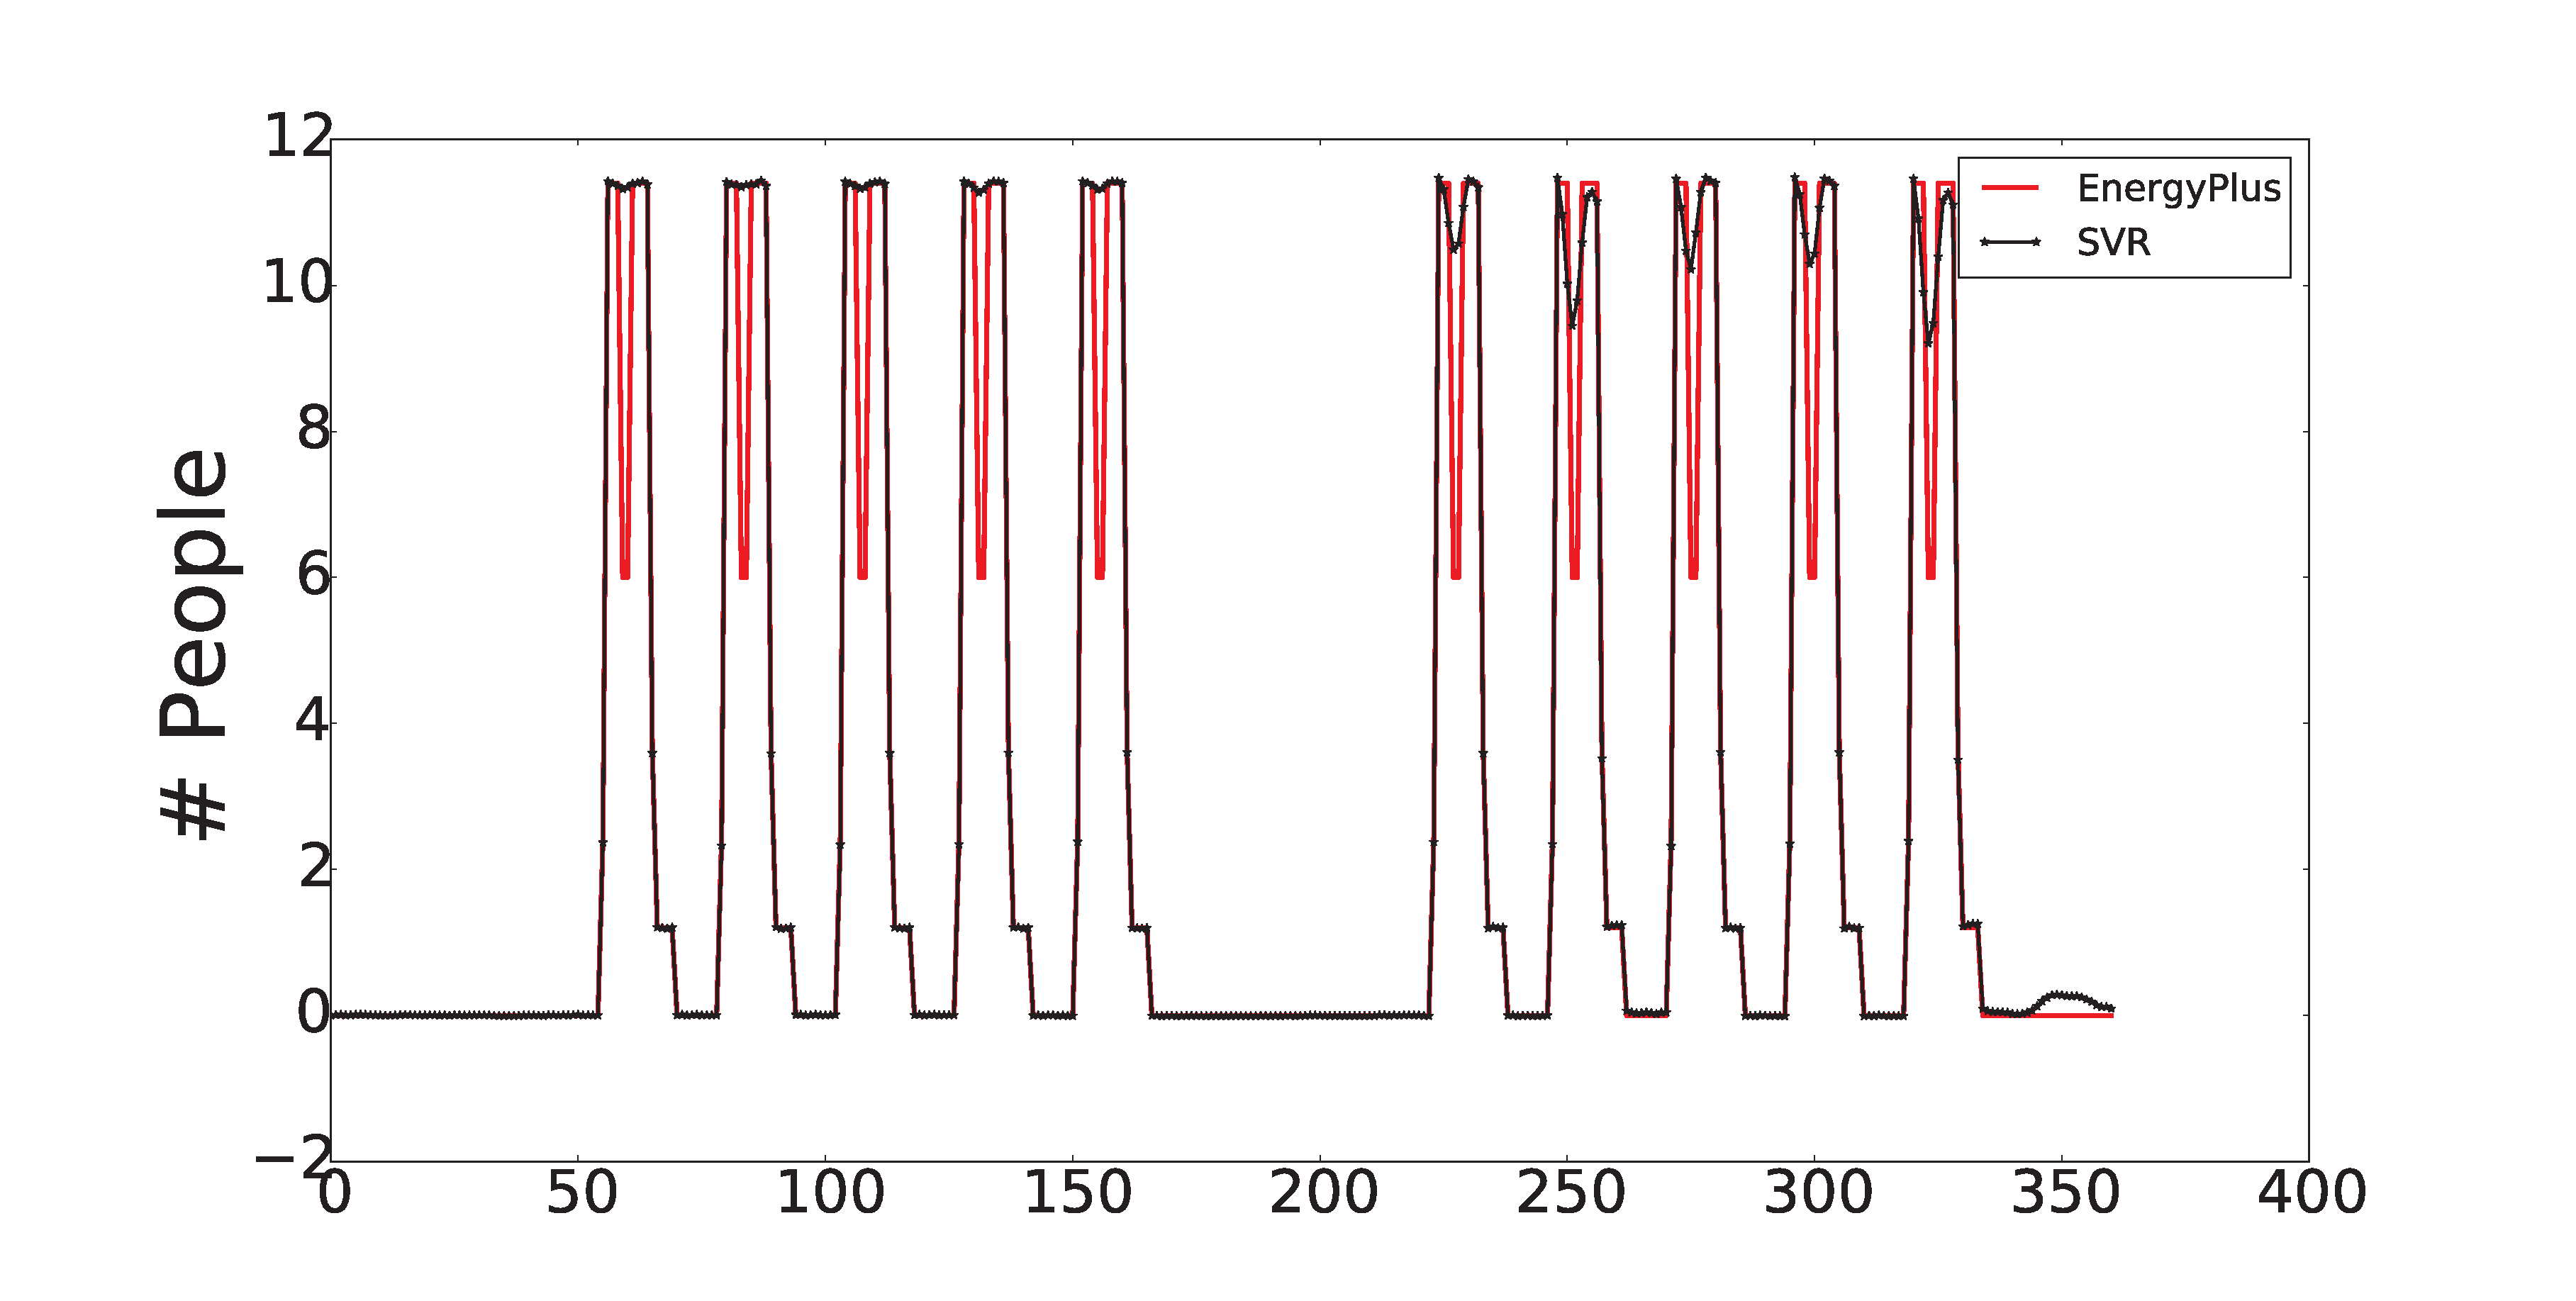
\includegraphics[width=5in]{./Pics/100C5Features.eps}
%\subcaption{}\label{fig:1b}
(b) 5 features.
\end{minipage}
\hfill
\caption{Occupancy estimation accuracy when $C$ equals 100 using SVR with 4
    features and 5 features. X-axis spans over 360 hours (15 days), sampled
    hourly.}\label{fig:compare1}
\end{figure}

\begin{figure}[h]
\begin{minipage}{\textwidth}
\centering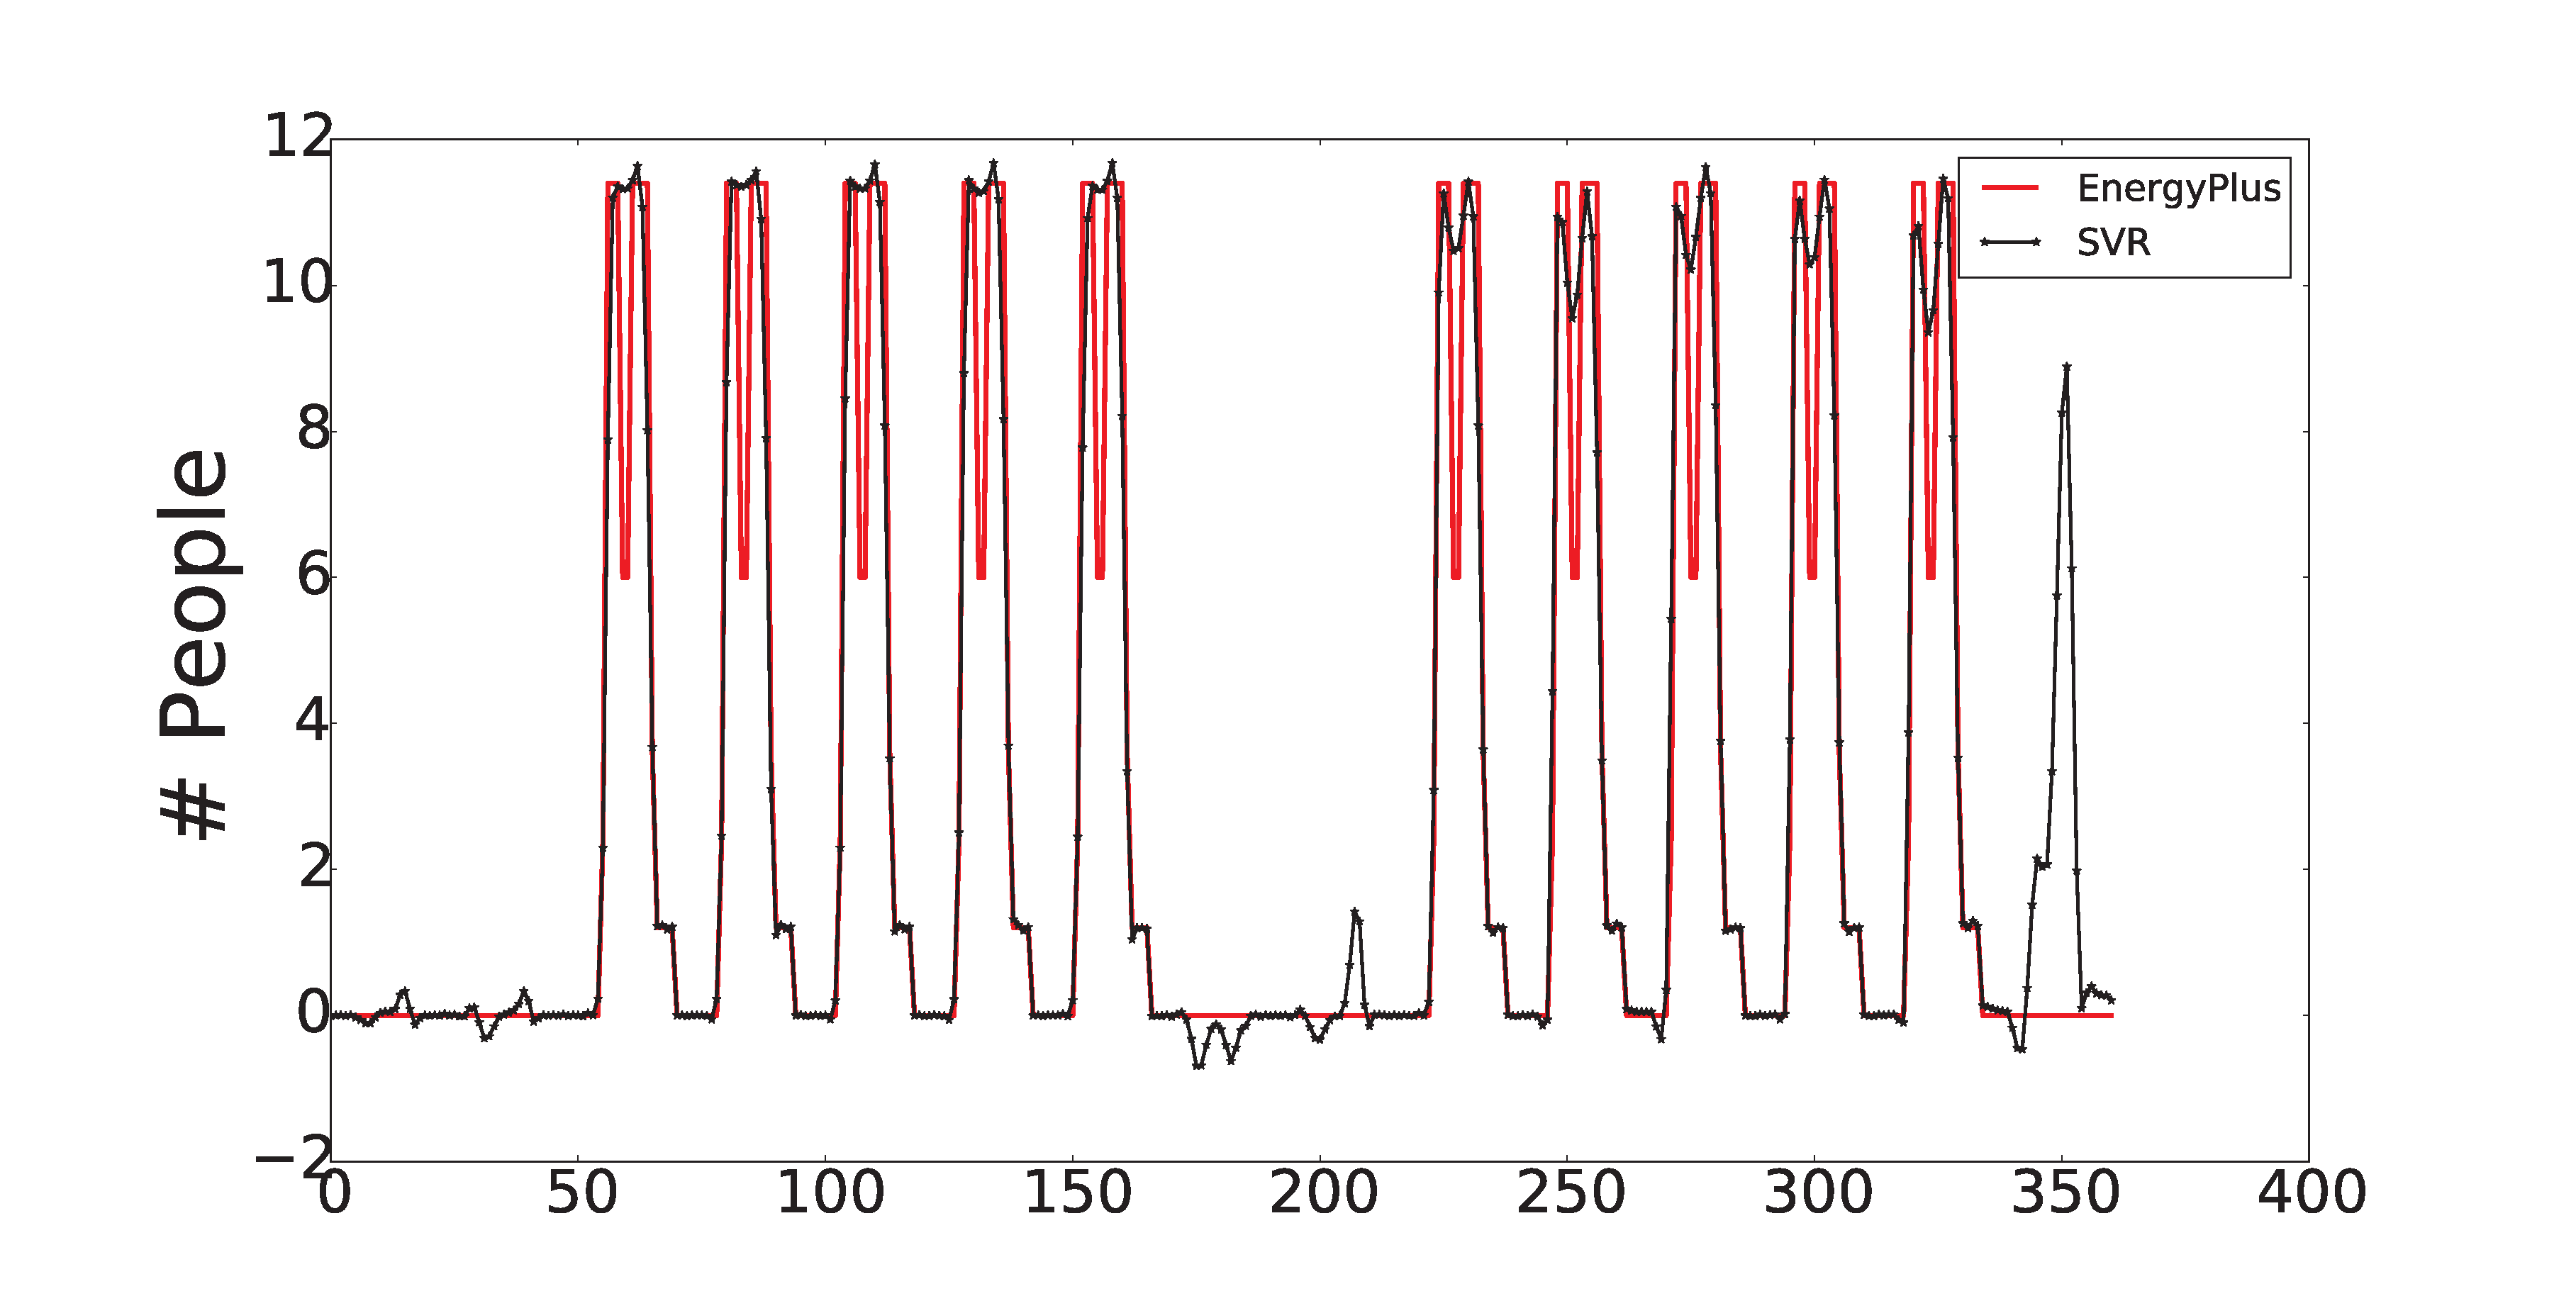
\includegraphics[width=5in]{./Pics/500C4Features.eps}
(a) 4 features.
\end{minipage}
\hfill

\vspace{3ex}

\noindent\begin{minipage}{\textwidth}
\centering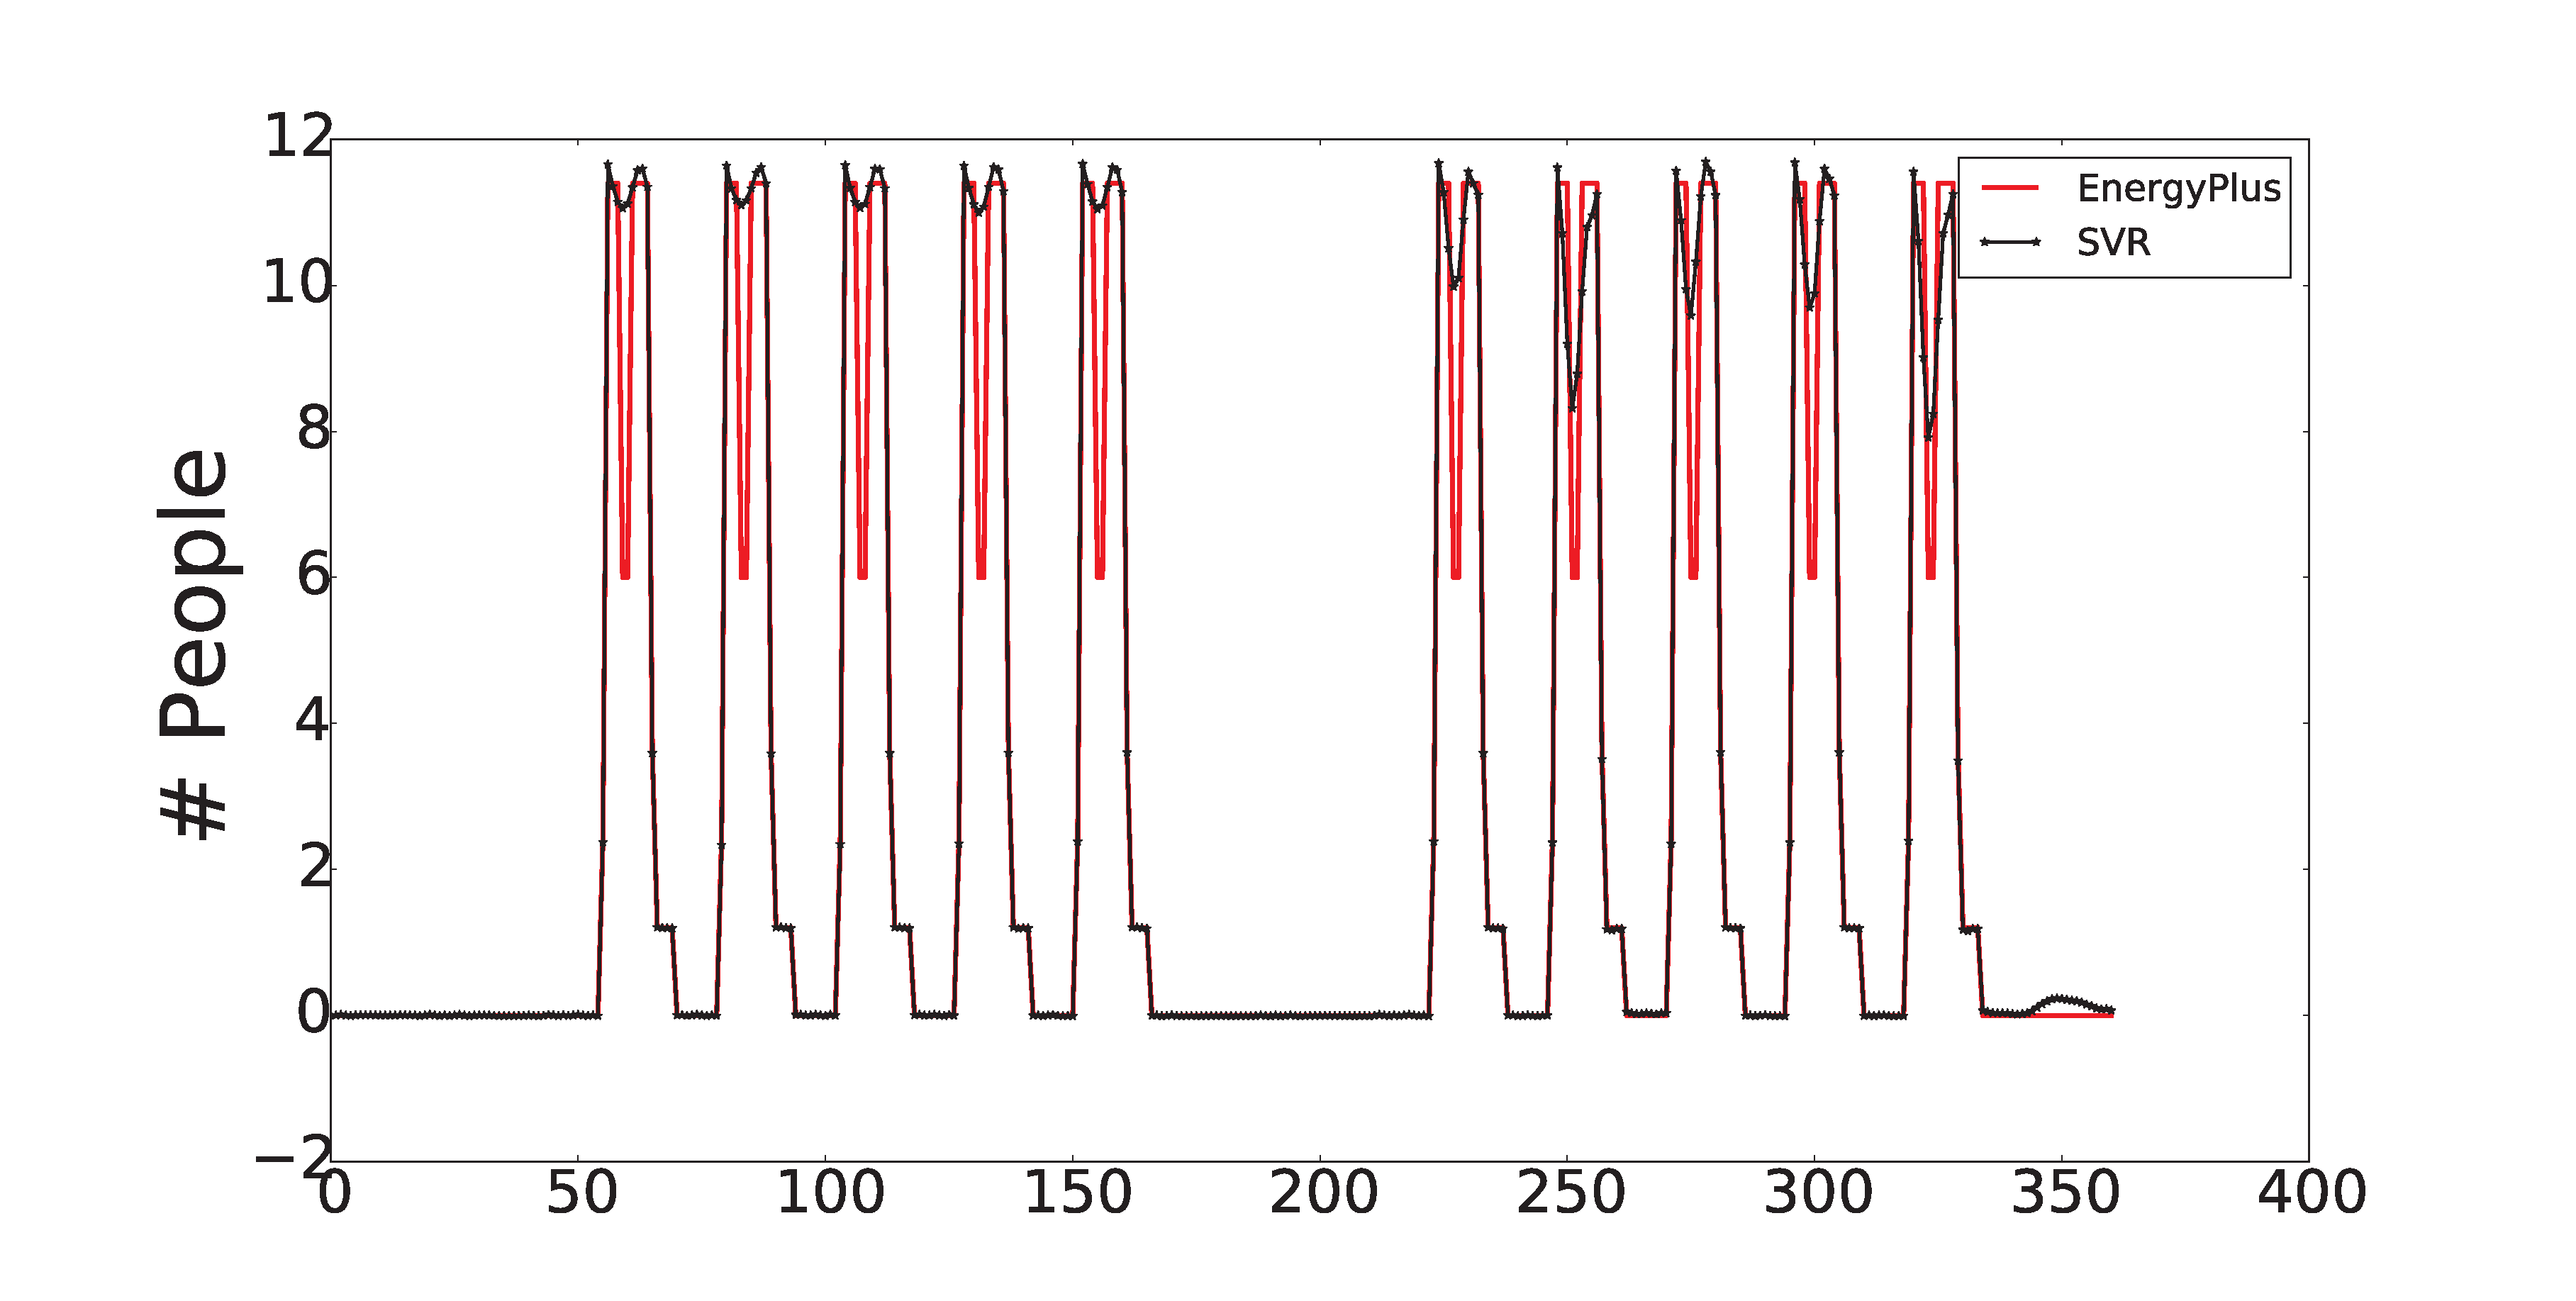
\includegraphics[width=5in]{./Pics/500C5Features.eps}
(b) 5 features.
\end{minipage}
\hfill
\caption{Occupancy estimation accuracy when $C$ equals 500 using SVR with 4
    features and 5 features. X-axis spans over 360 hours (15 days), sampled
    hourly.}\label{fig:compare2}
\end{figure}

\begin{figure}[h]
\begin{minipage}{\textwidth}
\centering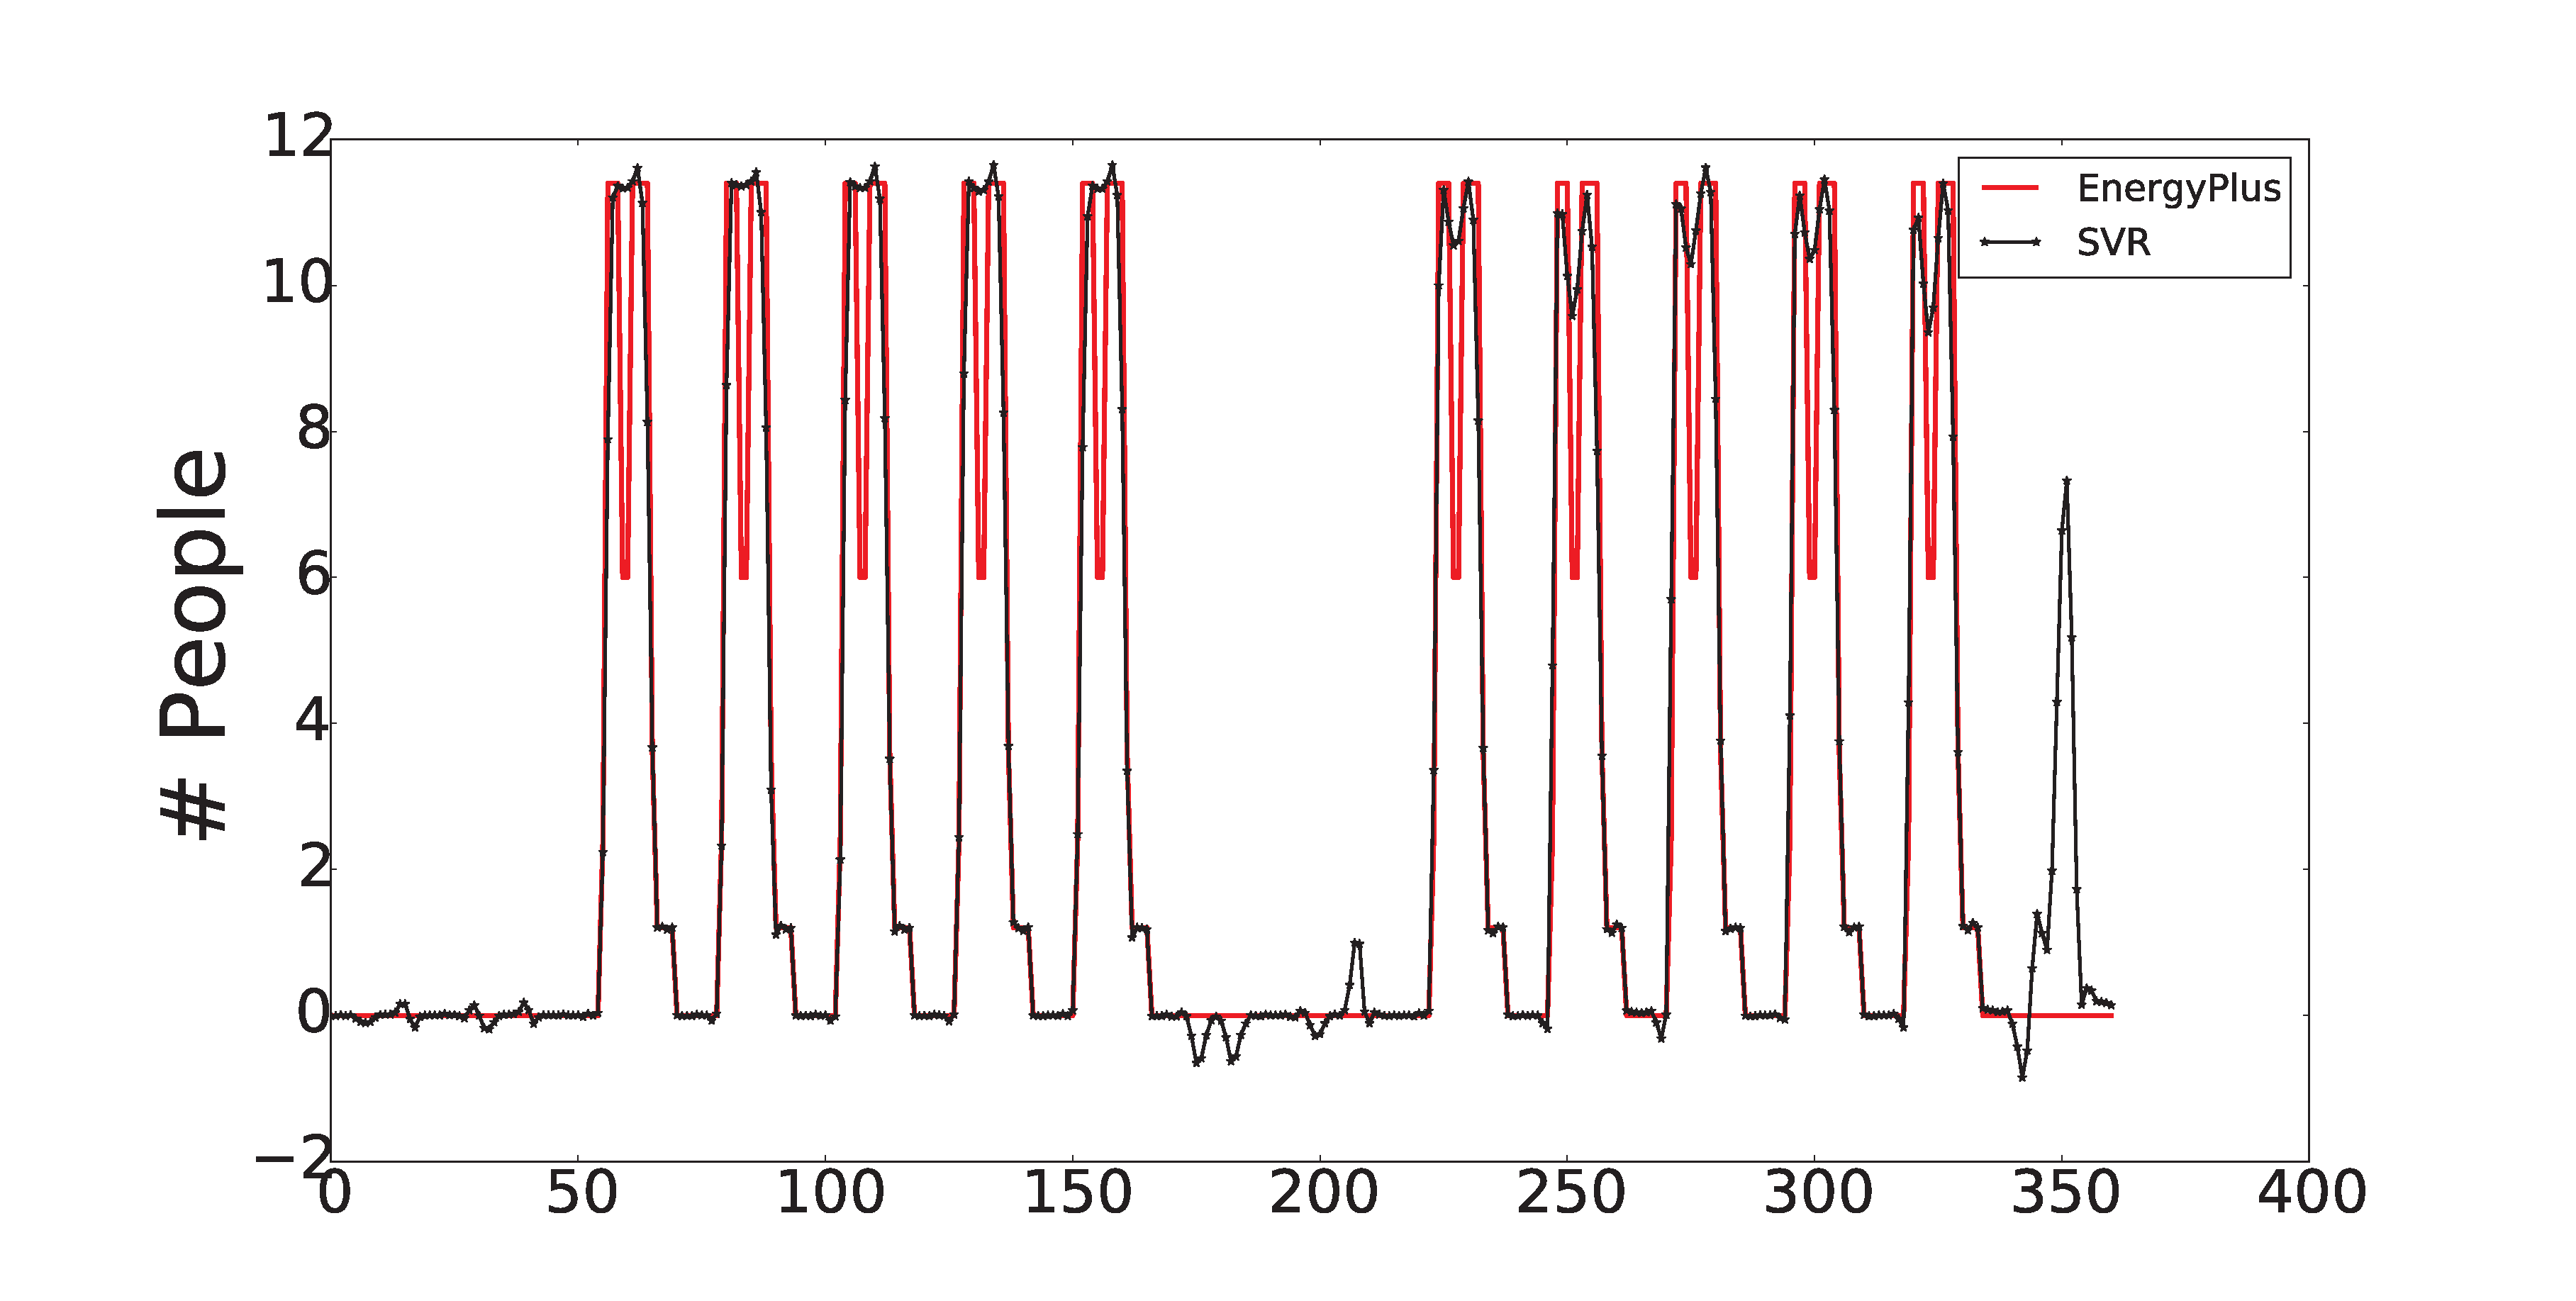
\includegraphics[width=5in]{./Pics/1000C4Features.eps}
(a) 4 features.
\end{minipage}
\hfill

\vspace{3ex}

\noindent\begin{minipage}{\textwidth}
\centering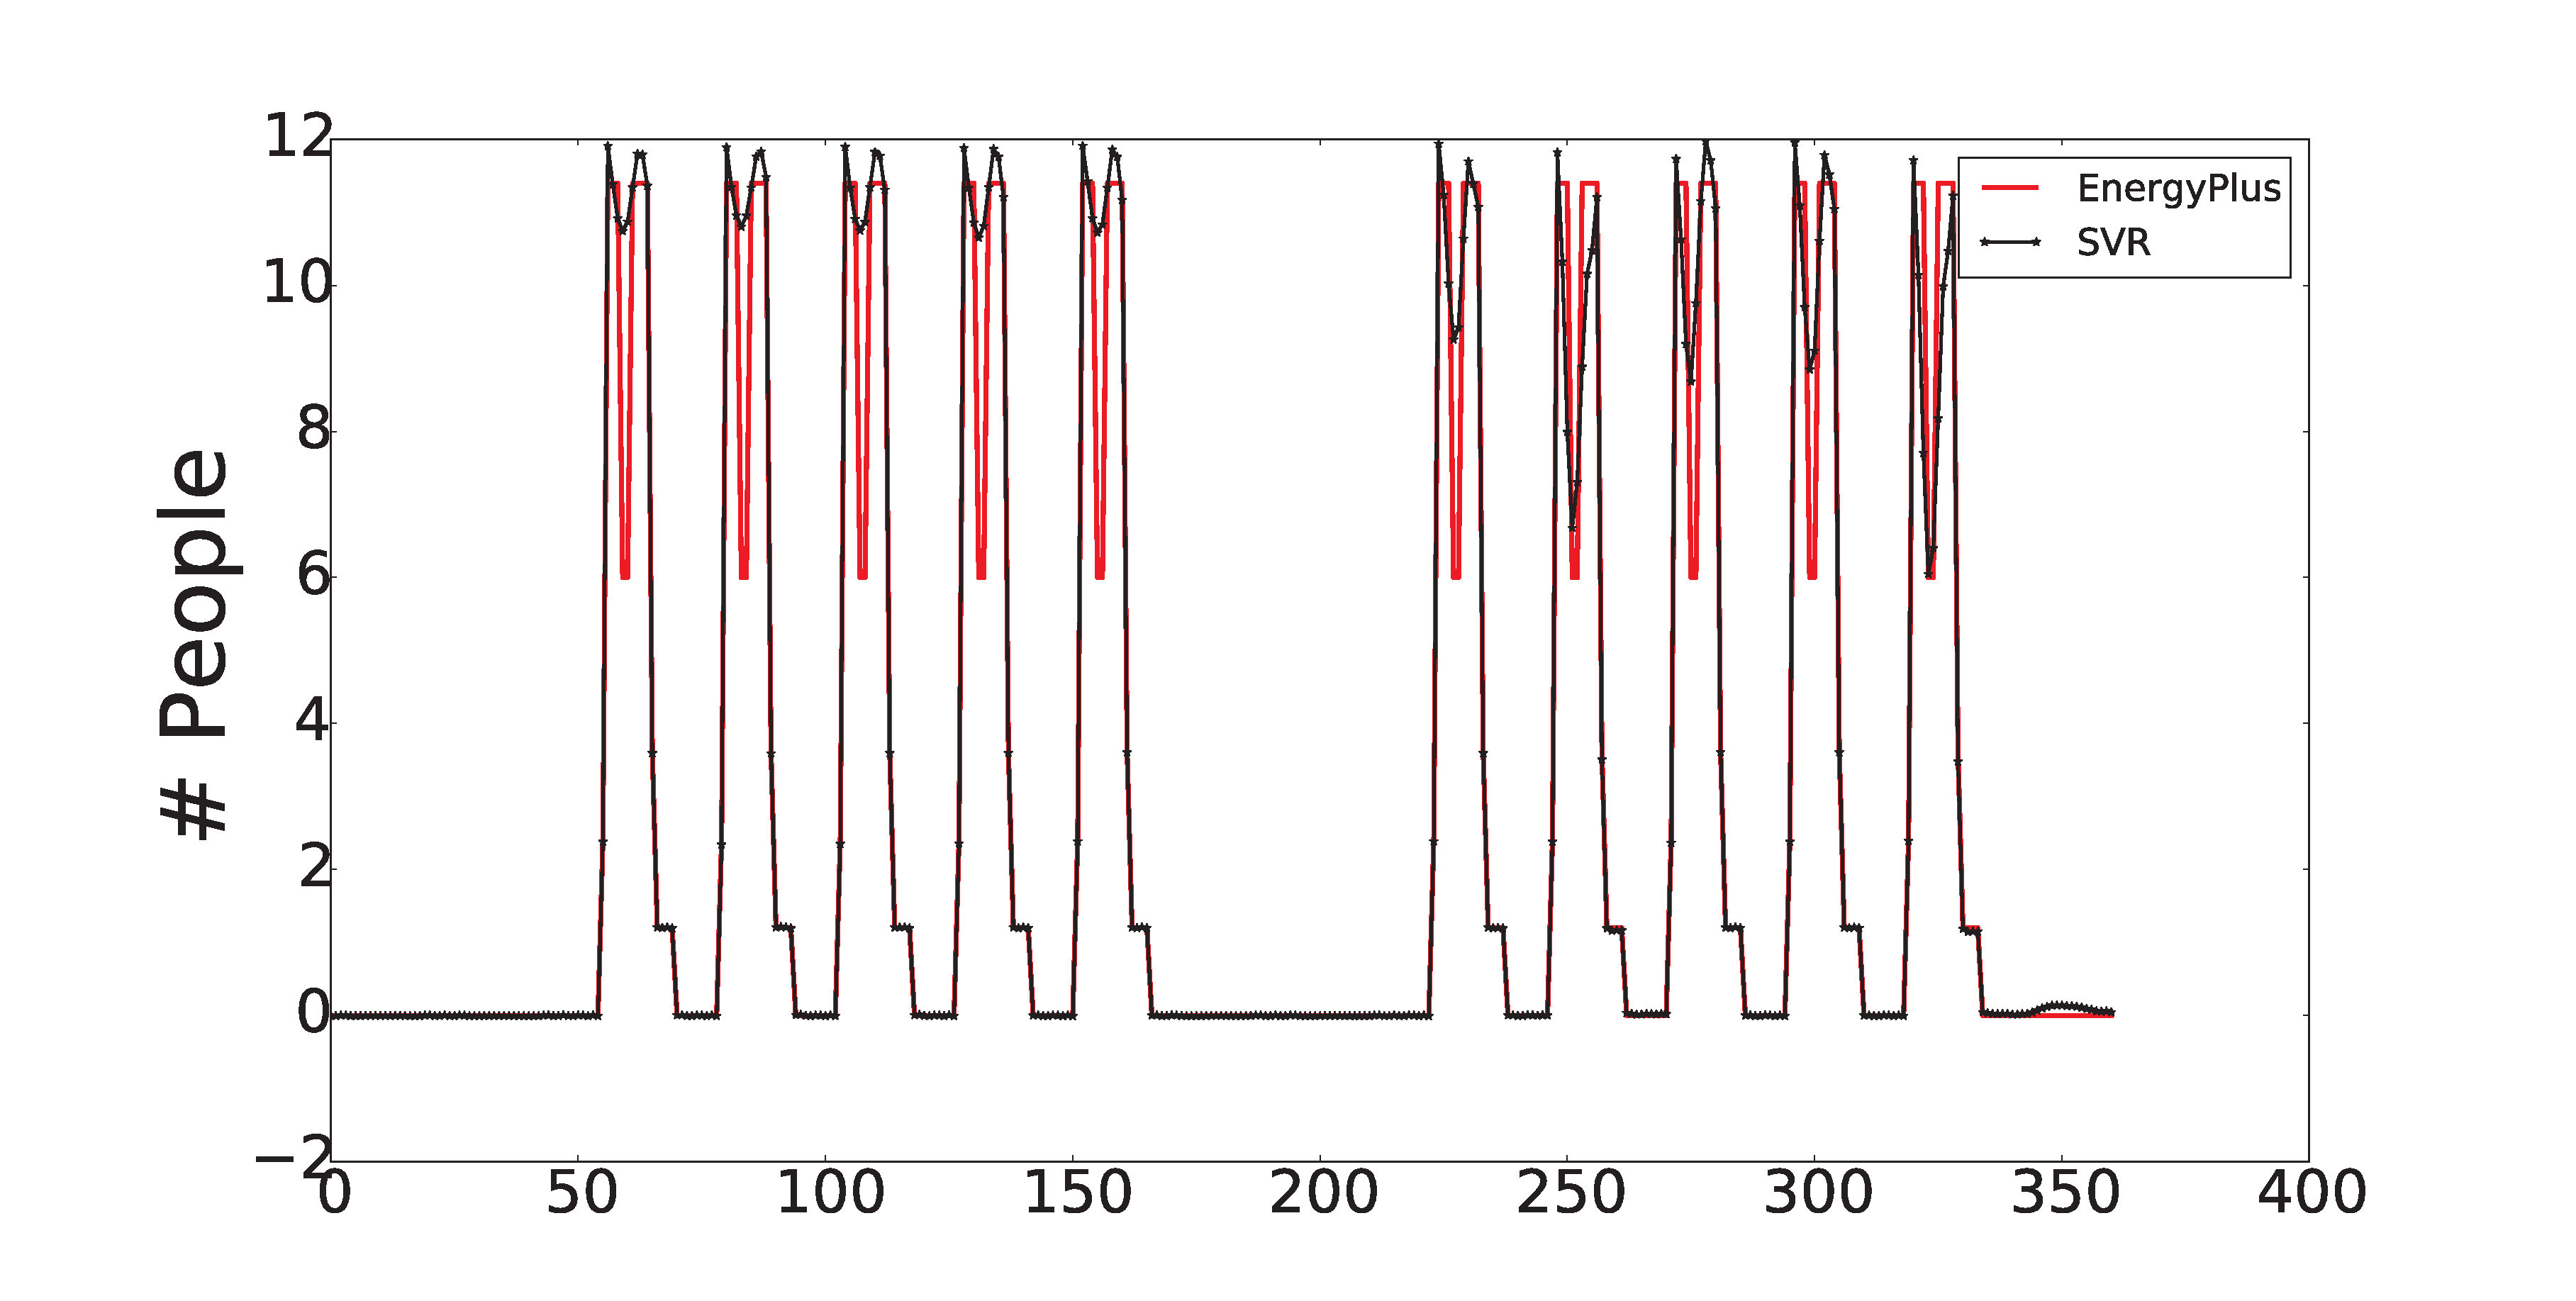
\includegraphics[width=5in]{./Pics/1000C5Features.eps}
%\subcaption{}\label{fig:1b}
(b) 5 features.
\end{minipage}
\hfill
\caption{Occupancy estimation accuracy when $C$ equals 1000 using SVR with 4
    features and 5 features. X-axis spans over 360 hours (15 days), sampled
    hourly.}\label{fig:compare3}
\end{figure}


In this part of the section, the process of achieving the best model we build
is revealed, and several figures of performance for models are displayed to
have a direct comparison for the model under different number of figures. The
figures mainly display the accuracy when applying 4 features or 5 features in
the model, and offers a clear comparison in those figures.

We now display the accuracy of applying 4 features or 5 features in the
proposed SVR model. To obtain the best parameter setting in the SVR model used
for occupancy detection, we need to constantly compare the gap between the
training and testing errors for the collected data sets by EnergyPlus. If the
gap of accuracy between training and testing errors are relatively large, which
means that this model is over-fitting on the training data. In accuracy on
training data implies that the model has a potential under-fitting. In this
situation, we need to adjust parameters to make the SVR-based model work
better.

We randomly pick out a 15-day period from the testing data set and compare it
to the genuine value generated by EnergyPlus. Large number of experiments in
this proposed SVR model shows that 0.01 is a stable-performing value for
$\varepsilon$. Fig. \ref{fig:compare1}, Fig. \ref{fig:compare2}, and Fig.
\ref{fig:compare3} show the simulation results of occupancy detection accuracy
of SVR model by using different numbers of features. To find a better
performance model, we set $C$ to be 100, 500, and 1000, respectively.
Simulation results show that the SVR model tends to become more complex when
the value of $C$ becomes larger, hence the goal of optimizing the SVR model is
to find the value of $C$ that is one better trade-off between under-fitting and
over-fitting. For the 5-feature model, it can be seen that the SVR model can
obtain better performance for occupancy detection when the value of $C$ varies
in the range from 10 to 1000.

The two sets of features provide different convenience in detecting to meet
different demand. The first set of features  can be relatively easily acquired
while the second set requests more efforts. The first set of feature only
requires data set that can be obtained from mathematical computation, whereas the
second set  requires light energy which is a set of statistics that needs more
effort to achieve. In terms of practical application, it is suggested to choose
the one that meets demand and gives the best convenience. However, further
improvement can be considered by building model revolving around absorbing the
current data set into the SVR model, which makes the model work as a dynamic
equation that is able to self-improved by newly absorbed data set and remain
more effectively according to the current circumstance. Most importantly, it is
suggested to choose the most efficient approach based on the facing situation,
after all, the model is able to fulfill ordinary demand in accuracy in
4-feature model. Further improvement is likely to happen if one considers
specific conditions for other office in detail.

\subsection{RNN Based Occupancy Detection}
\label{sec:rnn-method}

In this section, the Elman's recurrent neural network as shown in
Fig.~\ref{fig:elman} is used for occupancy detection in a building.

\subsubsection{Experiments}
EnergyPlus takes outdoor thermal factors (such as ambient temperatures and solar
factors), people occupancy and HVAC related powers as input, and produce the
temperatures of rooms as its output. People occupancy is in unit of number of
people, which maybe decimal as it represents average people count over a short
time span. We treat all the data used and produced by EnergyPlus equally as
real-world factors, regardless they were inputs or outputs of EnergyPlus. In the
occupancy estimation work, we select data from those real-world factors, feed
them into the recurrent neural network, and try to get estimated occupancy from
it.

We use EnergyPlus to simulate the room thermal behavior in a year, using various
inputs including occupancy information. We collect the inputs and outputs (room
temperatures) of EnergyPlus simulation, which is discretized into hourly data
points, to train ELNN. Given the simulated data
provided by EnergyPlus, as shown in Fig.\ref{fig:data-flow}, we feed selected
channels of ambient factors and other power data, along with room temperatures,
into ELNN as input. We use estimated and real
occupancy to drive the training process. We will configure two different
selected datasets: one uses ambient factors and room temperatures only, another
dataset uses ambient factors, room temperatures and HVAC cooling/heating
powers. The output of ELNN has multiple channels, which are
respectively each room's estimated people occupancy.

\begin{figure}[t]
    \centering
    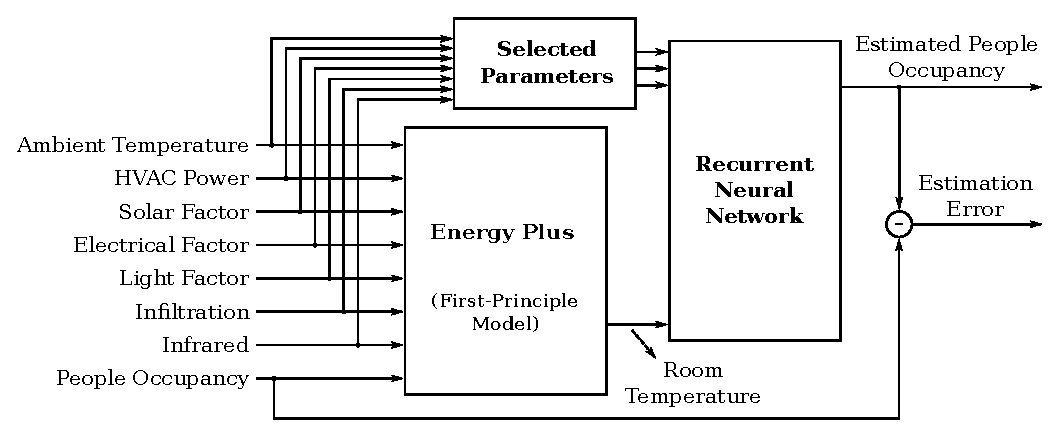
\includegraphics[width=0.9\columnwidth]{figs/rnn/data-flow.eps}
    \caption{Data configuration of Elman's recurrent neuron network.}
    \label{fig:data-flow}
\end{figure}

In practical smart-building applications, room temperatures are easy to acquire
from the installed sensors. Ambient temperature, solar factors are also
relatively easier to be acquired or calculated. While other factors, such as
HVAC cooling or heating powers, electrical equipment powers and air
infiltrations, need more instruments to per-room estimate in real-time. Because
of these limitations, we select two different sets of real-world factors as the
network input and compare the occupancy evaluation accuracy:
\begin{enumerate}
    \item Input includes ambient temperature, solar factors and room
    temperatures only. This will be referred as configuration I.

    \item Input includes ambient temperature, solar factors, room temperatures
    and HVAC cooling\slash{}heating powers. This will be referred as configuration II.
\end{enumerate}
With different factors as network inputs, we also configure the recurrent
neural network with different hidden recurrent layers varying from one to
three ($k=1,2,3$), to compare the estimation accuracies. We divide the one year
simulation data into 12 months. Months 1--3, 5--7, 9--11 are used for training;
months 4, 8, 12 are used for validating the trained networks.

We evaluate the performance (mainly accuracy) of the
proposed occupancy estimation method on a dataset of one year using
the building example shown in Fig.~\ref{fig:5zone}.  We picked a
15-day data subset starting from the 3rd Sunday in August to be
plotted in Fig.~\ref{fig:one-layer} and Fig.~\ref{fig:two-layer}. We
report the validation errors for one-layer and two-layer networks
since they are non-trivial and more noticeable. These figures show
that the occupancy estimation of room 1, among all the 5 rooms in this
case, having similar error situations.



\begin{figure}[h]
\begin{minipage}{\textwidth}
\centering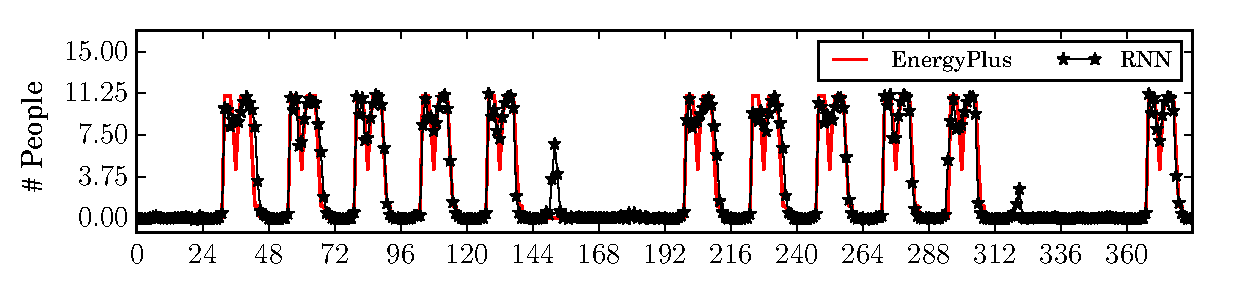
\includegraphics[width=5in]{figs/results/1LRoomTOnlyDPFAugW3-4}
%\subcaption{}\label{fig:1a}
Conf. I: Ambient factors and room temperatures.
\end{minipage}
\hfill

\vspace{3ex}

\noindent\begin{minipage}{\textwidth}
\centering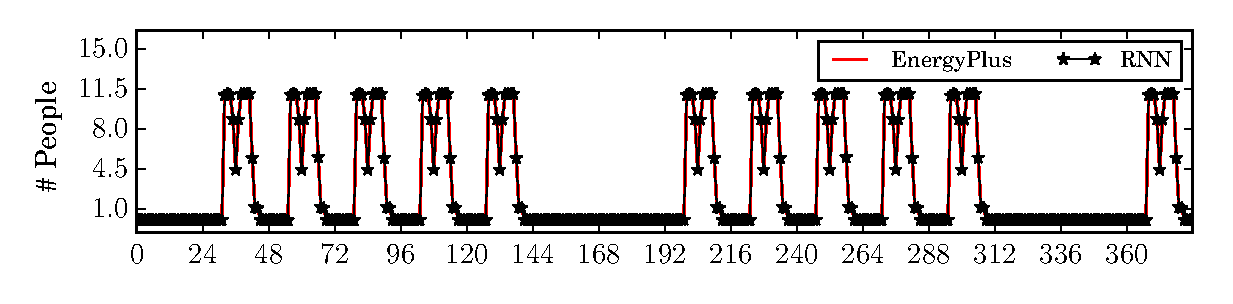
\includegraphics[width=5in]{figs/results/1LAmbHVACDPFAugW3-4}
Conf. II: Ambient factors, room temperatures and HVAC powers.
\end{minipage}
\hfill
    \caption{Occupancy estimation accuracy using one-layer recurrent neural
    network with input configurations I and II. X-axis
    spans over 384 hours (16 days), sampled hourly.}\label{fig:one-layer}
\end{figure}

\begin{figure}[h]

\begin{minipage}{\textwidth}
\centering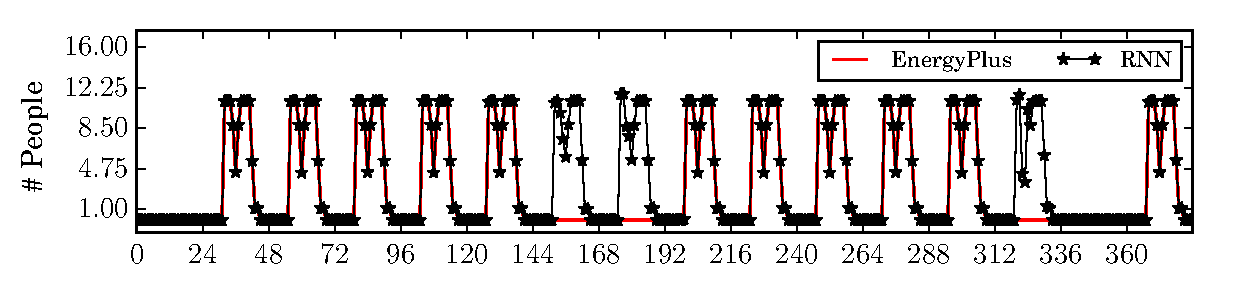
\includegraphics[width=5in]{figs/results/2LRoomTOnlyDPFAugW3-4}
Conf. I: Ambient factors and room temperatures.
\end{minipage}
\hfill

\vspace{3ex}

\noindent\begin{minipage}{\textwidth}
\centering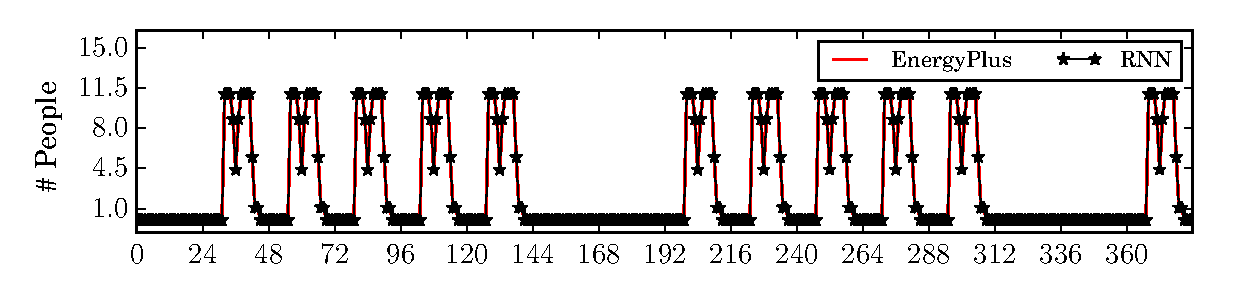
\includegraphics[width=5in]{figs/results/2LAmbHVACDPFAugW3-4}
Conf. II: Ambient factors, room temperatures and HVAC powers.
\end{minipage}
\hfill
\caption{Occupancy estimation accuracy using two-layer recurrent neural network
    with input configurations I and II. X-axis spans over
    384 hours (16 days), sampled hourly.}\label{fig:two-layer}
\end{figure}


\subsubsection{Analysis}
The training and validation error statistics are shown in
Table~\ref{tab:terr-stat} and Table~\ref{tab:verr-stat}, respectively.
In the input configuration I, we use ambient and room temperatures
only as the inputs (this is similar to situation in which we only know
temperature information from thermal sensors); in the input
configuration II, we use ambient, room temperatures and HVAC
cooling/heating powers as the inputs (in case we know more information
about a building).

At every sample point, estimation error $e_i$ is calculated using
$e_i=\left|p_i^{\text{RNN}}-p_i^{\text{EP}}\right|$, where
$p_i^{\text{RNN}}$ is people occupancy estimated by the RNN and
$p_i^{\text{EP}}$ is referencing value used in EnergyPlus. Note that we may
have zero people in a room (the occupancy value $p_i^\text{EP} = 0$), so
no relative errors are used. Also, occupancy values can be
non-integer numbers as the estimated number of people in a room is a
average number in a period.

In Table~\ref{tab:terr-stat} and Table~\ref{tab:verr-stat}, average
error is calculated using $\frac1n\sum_ne_i$; maximum error is
calculated using $\max\{e_i\}$; error rate is the number of points
where $e_i>0.5$. We discuss the estimation accuracy separately about
data configurations I and II.

\begin{table}[t]
    \centering
    \begingroup
    \setlength{\tabcolsep}{3.6pt} 
    \begin{tabular}{lrrcrrcrr}
        \toprule
        & \multicolumn{2}{c}{1 Hidden Layer} && \multicolumn{2}{c}{2 Hidden Layers} && \multicolumn{2}{c}{3 Hidden Layers}\\
        \cmidrule{2-3} \cmidrule{5-6} \cmidrule{8-9}
        & Conf.~I & Conf.~II && Conf.~I & Conf.~II && Conf.~I & Conf.~II\\
        \midrule
        Avg.~error & 0.451      & 0.0149    && 0.00635   & 0.00643   && 0.0308      & 0.0291    \\
        Max.~error & 12.6       & 0.544     && 0.284     & 0.141     && 0.807       & 0.788     \\
        Error rate & 20\%       & 0.0061\%  && 0.00\%    & 0.00\%    && 0.082\%     & 0.015\%   \\
        \bottomrule
    \end{tabular}
    \endgroup
    \caption{Training errors of three Elman architectures using two
        different input configurations.}
    \label{tab:terr-stat}
\end{table}

\begin{table}[t]
    \centering
    \begingroup
    \setlength{\tabcolsep}{3.6pt} % Default 6pt
    \begin{tabular}{lrrcrrcrr}
        \toprule
        & \multicolumn{2}{c}{1 Hidden Layer} && \multicolumn{2}{c}{2 Hidden Layers} && \multicolumn{2}{c}{3 Hidden Layers}\\
        \cmidrule{2-3} \cmidrule{5-6} \cmidrule{8-9}
        & Conf.~I & Conf.~II && Conf.~I & Conf.~II && Conf.~I & Conf.~II\\
        \midrule
        Avg.~error & 0.538      & 0.0175    && 0.153     & 0.00560   && 0.0439      & 0.0340    \\
        Max.~error & 17.8       & 2.82      && 18.1      & 0.288     && 11.4        & 1.66      \\
        Error rate & 21\%       & 0.11\%    && 2.4\%     & 0.00\%    && 0.71\%      & 0.38\%    \\
        \bottomrule
    \end{tabular}
    \endgroup
    \caption{Validation errors of three Elman architectures using two
        different input configurations.}
    \label{tab:verr-stat}
\end{table}

In data configuration I, one-layer network suffers from under-fitting
problem (about 20\% data points have errors greater than 0.5). This is
because the network needs more internal status to have the capability
to estimate the people occupancy only use room and ambient
temperature.  As we increasing the number of network layers,
estimation accuracy improves (error rate 2.4\% for 2-layer and 0.71\%
for 3-layer). Experiment results show that the RNN is able to estimate
people occupancy only with ambient and room temperatures with a good
accuracy (lower than 1\%).

In the configuration II, we provide more information (HVAC powers)
for the occupancy training process than the configuration I. As a
result, the ELNN with only two hidden recurrent layers can
already perform quite well (no points having error grater than 0.5
were observed in the one-year data). As network size grows (up to 3),
the estimation error grows (0.38\%), but stays in acceptable level.

\subsection{Comparison Between SVR and RNN}
\label{sec:comparison_svr_rnn}

\begin{figure}[!h]
\centering
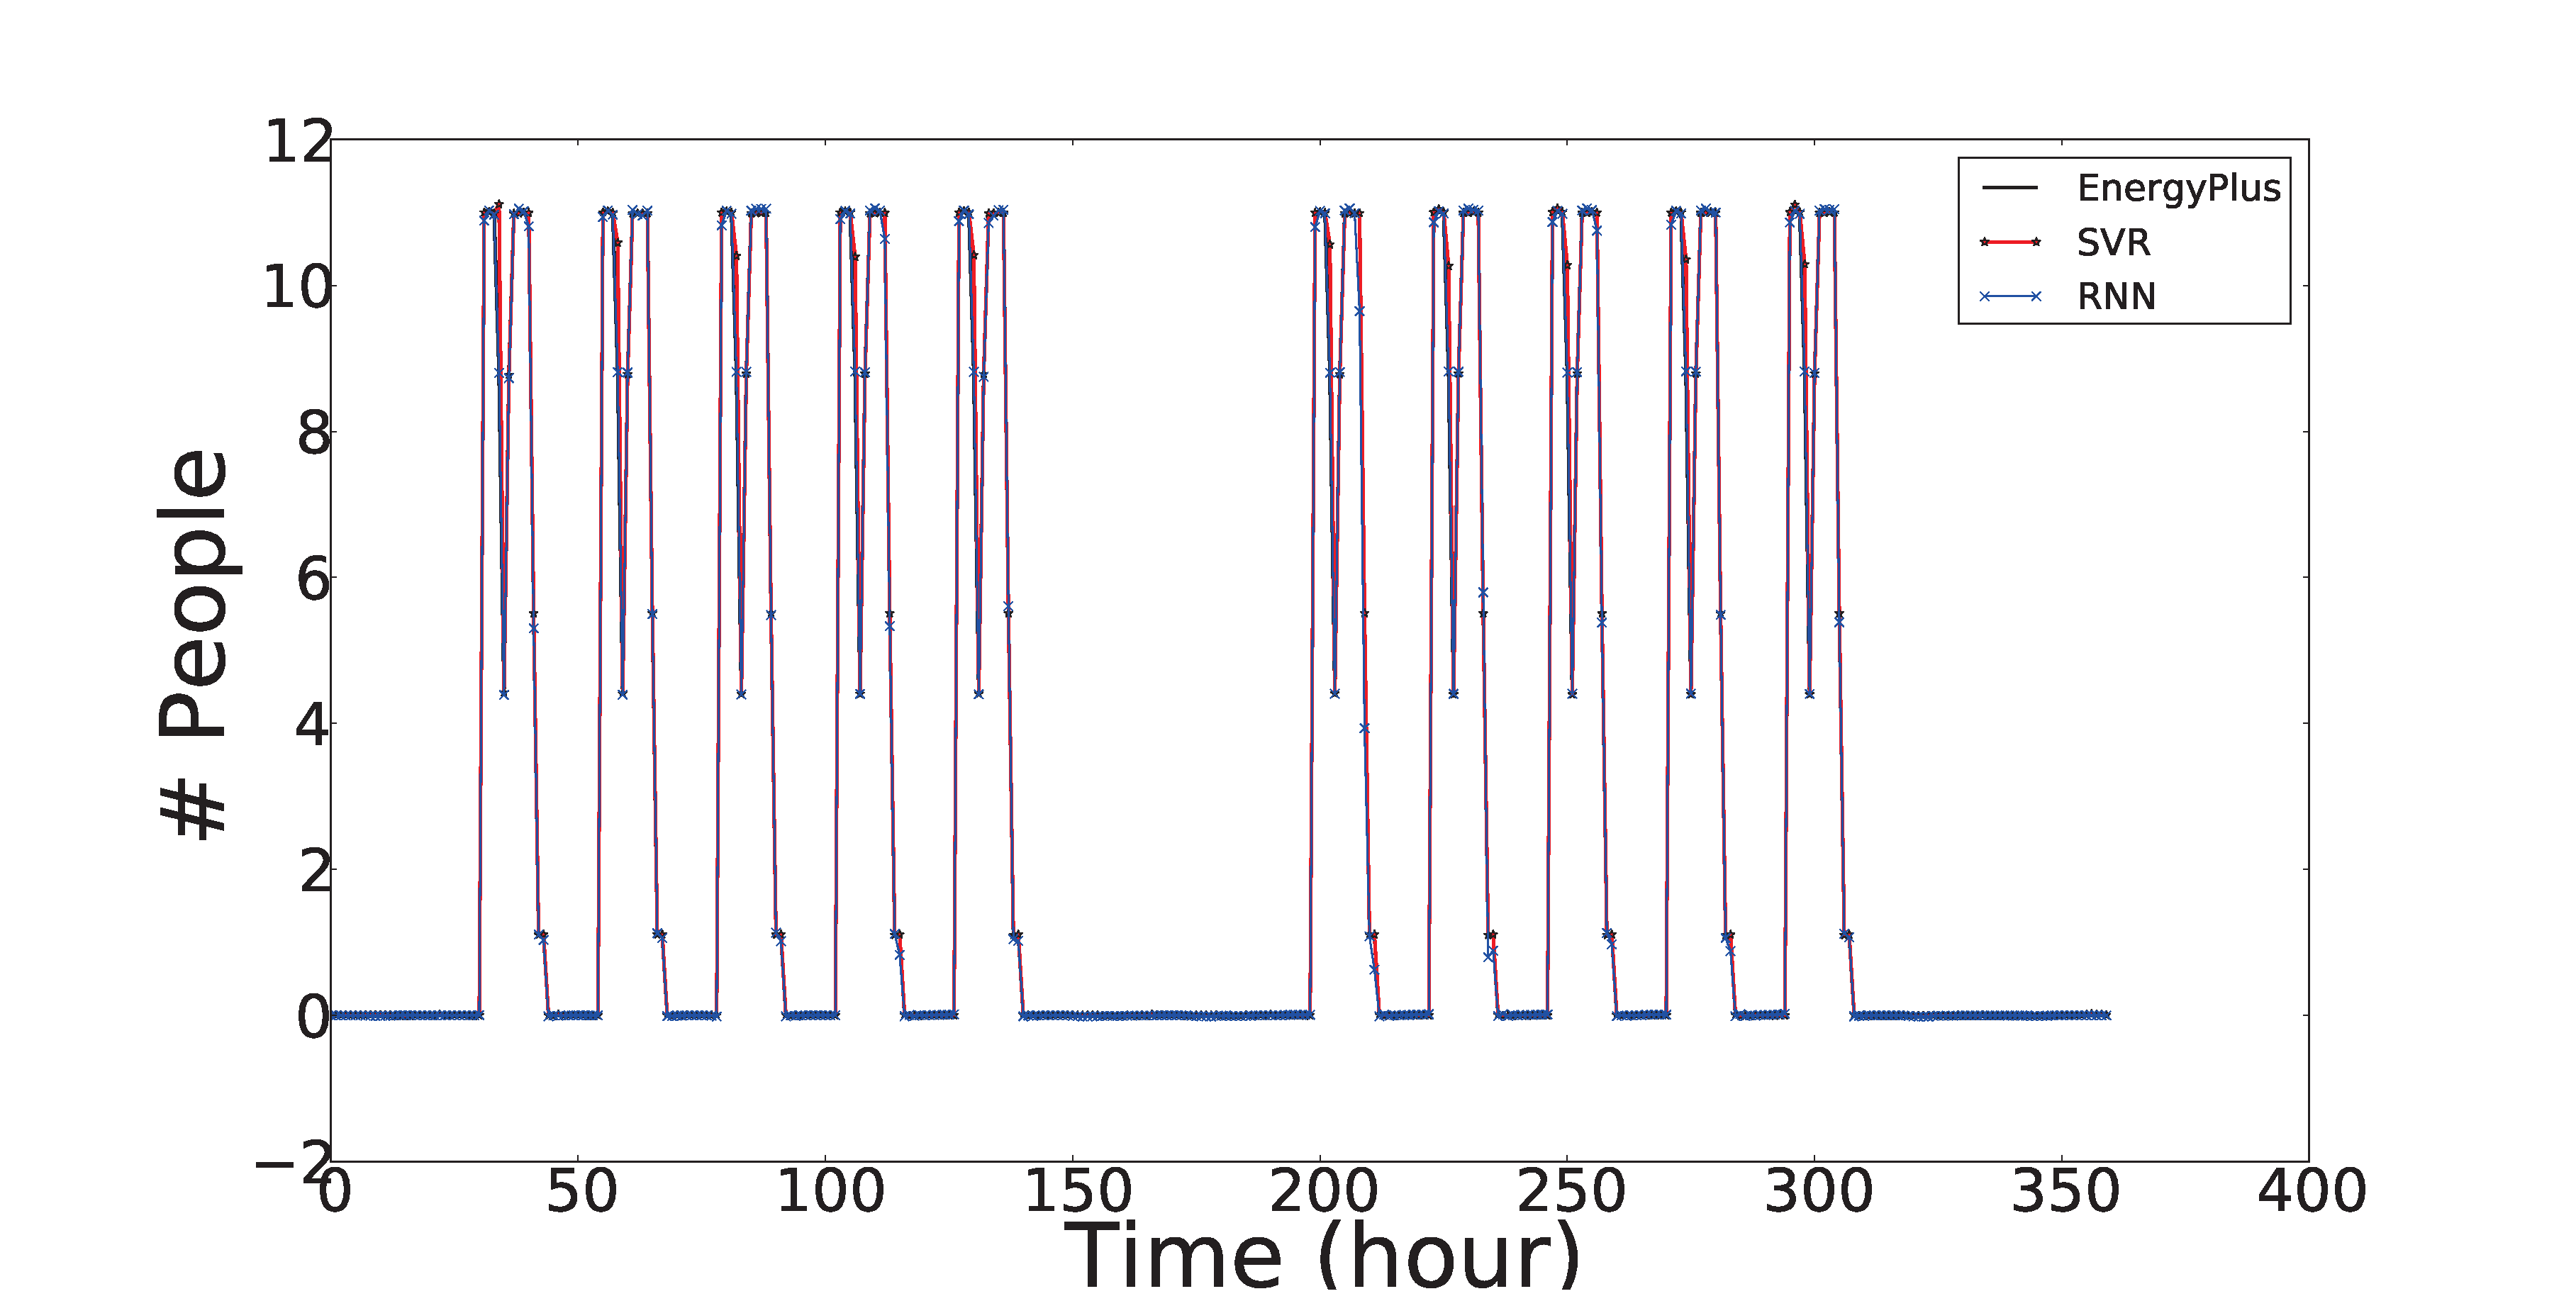
\includegraphics[width=5in]{./Pics/comparison.eps}
\caption{Comparison between SVR and RNN in occupancy detection.}
\label{fig:comparison}
\end{figure}

In this section, we compare the accuracy and characteristics of the
occupancy detection result respectively from SVR and RNN. It should be noted that the same
features are used for the two different models in order to make a fare comparison.
Fig.~\ref{fig:comparison} shows the result in which the black curve
stands for the original outcome, the red curve stands for the SVR
outcome, and the blue curve stands for the RNN outcome.  Those results
are generated based on the same features and number of data, which
means, the different results shown in the figure are only influenced
by the models. From the figure, we can see that the results from both
methods agree well with the original curves.  Furthmore, we obseve
there is a small fluctuation in Max.~error when the SVR model is
applied. This indicates the maximum error of the SVR model will stay
at a stable range when the features of the model are slightly
changed. In comparison, Max.~error of the RNN model is relatively more
sensitive. The Max.~error may double, triple, or rapidly diminishes
when the features of the model is changed. This phenomenon is also
observed in the Avg.~error. The numeric value of Avg.~error swings
more for the RNN model than for the SVR model under the situation that
the features are changed. This could imply the two different
characteristic behaviors of the two models, which gives the user the
flexibility to apply for those two models. The SVR model is used when
the features of a model will change from every now and then, in order
to keep the detection precision at a stable range. The RNN model is applied
when features are not changed in a real context, which possess a even higher
precision in detecting occupancy compared to SVR.
Comparing to 92\% detection accuracy in \cite
{dong2014real}, as shown in Figure \ref{fig:accuracy-comparison}, moderately
configured SVR and RNN models can achieve occupancy detection accuracy higher
than 96\%.

\begin{figure}[h]
    \centering
    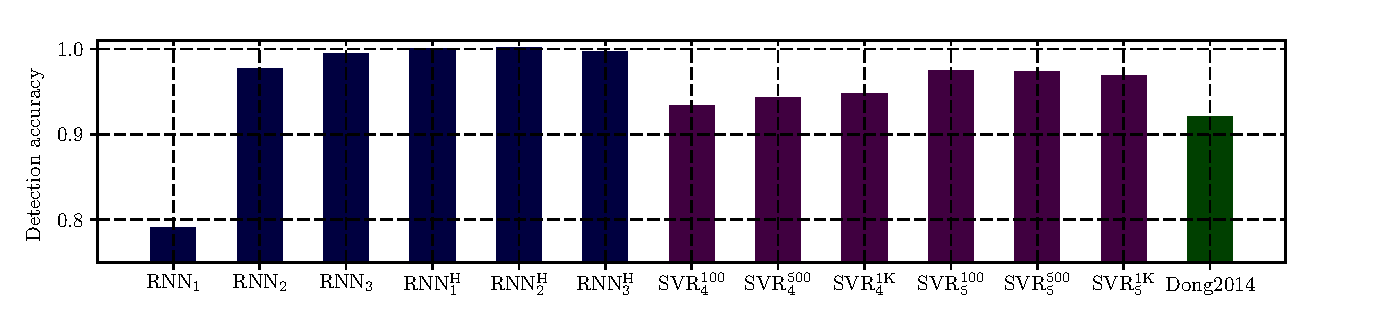
\includegraphics[width=\textwidth]{./figs/results/results_compare.eps}
    \caption{Occupancy detection accuracy using SVR and
    RNN. (Explanation for the X-axis labels: subscript and superscript of RNN
    denotes number of hidden layers and awareness of HVAC; subscript and
    superscript of SVR denotes number of features and $C$ value.)}
    \label{fig:accuracy-comparison}
\end{figure}

We remark that since SVR has great
  generalization ability and can guarantee to find the local minimum,
  SVR can perform well for time series analysis for occupancy
  detection. RNN can also be used for a time series prediction problem
  as the data configuration for RNN includes time steps. The most
  important features related to occupancy behavior in a building are
  used in the machine learning methods. These features covers all
  major thermal-related aspects to be coupled with the human
  activity. As a result, occupancy behavior can be accurately
  determined by using the selected machine learning methods with time
  series analysis.

